\section{Laboratory work implementation}

\subsection{Tasks and Points}

- Fiecare din membrii echipei va lucra pe propriul branch in git, iar una din persoane va avea grija sa faca merge cu master; \\
\indent 
- Proiectul se poate afla doar in repozitoriul unui membru al echipei; \\
\indent 
- Dezvoltarea unei aplicatii: Mobile;

\subsection{Analiza lucrarii de laborator}
\selectlanguage{russian}
В ходе данной лабораторной работы было разработано приложение, реализующее функционал записной книжки. Работа была выполнена совместо с Русу Дмитрием TI-145.\\
\indent 
В мою часть задания входило: создание классов Utils, DBHelper, BitmapWorkerTask и Person.\\
\indent 
DBhelper - вспомогательный класс, для использования Базы Данных. В Базе Данных хранится Имена, Изображения и номер контакта. Класс Utils включает в себя 2 метода: для получения размеров картинки ( не загружая ее ) и подсчета во сколько раз ее можно уменьшить, без потери качества. BitmapWorkerTask - проверяет, есть ли картинка в кеше, если ее нет в кеше, то загружает из базы данных. Person - структура, которая включает поля с информацией о пользователе.\\
\indent 
Коды можно просмотреть на репозитории 



\subsection{Imagini}

\begin{figure}[h]
	\center{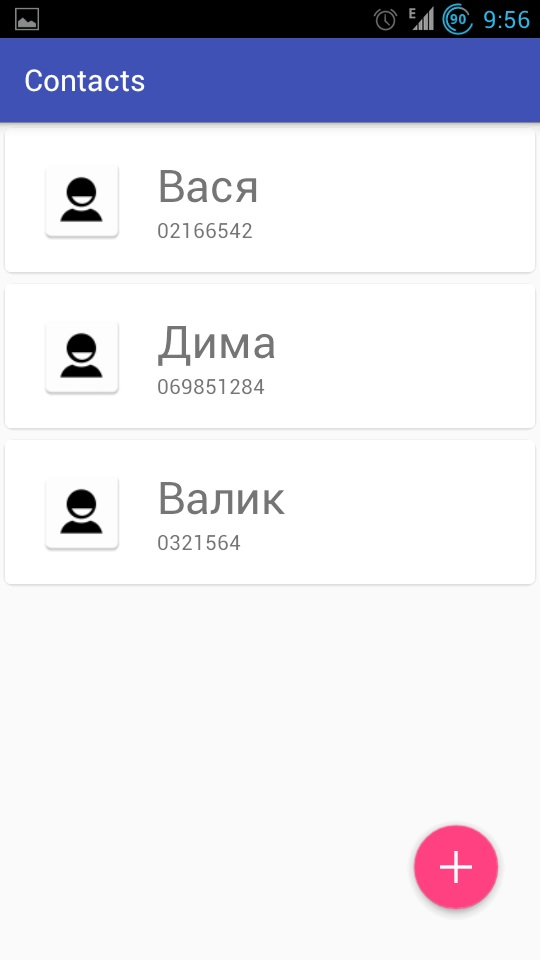
\includegraphics[width=1\linewidth]{images/1.jpg}}
	\caption{Заглавное меню}
	\label{ris:image}
\end{figure}
\hfill
\begin{figure}[h]
	\center{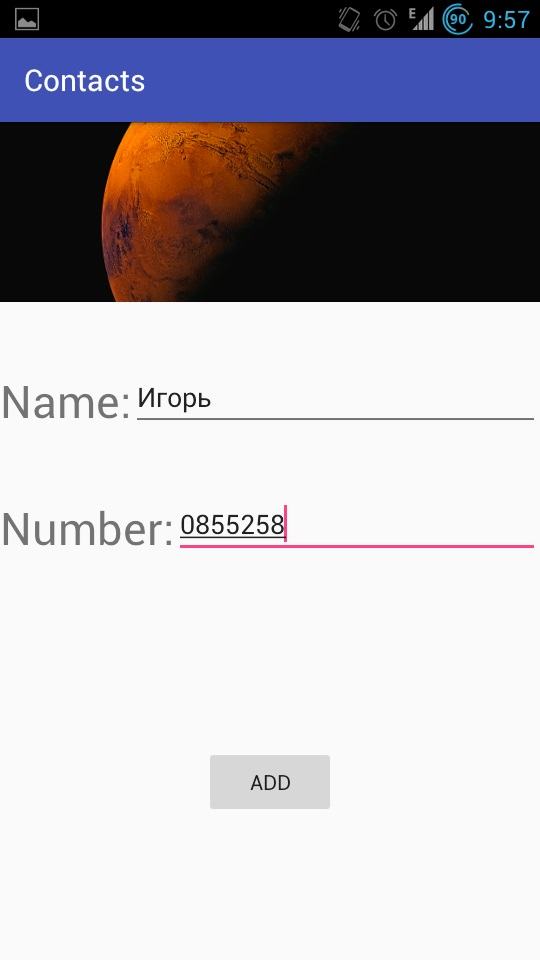
\includegraphics[width=1\linewidth]{images/2.jpg}}
	\caption{Добавление контакта в БД}
	\label{ris:image}
\end{figure}
\hfill
\begin{figure}[h]
	\center{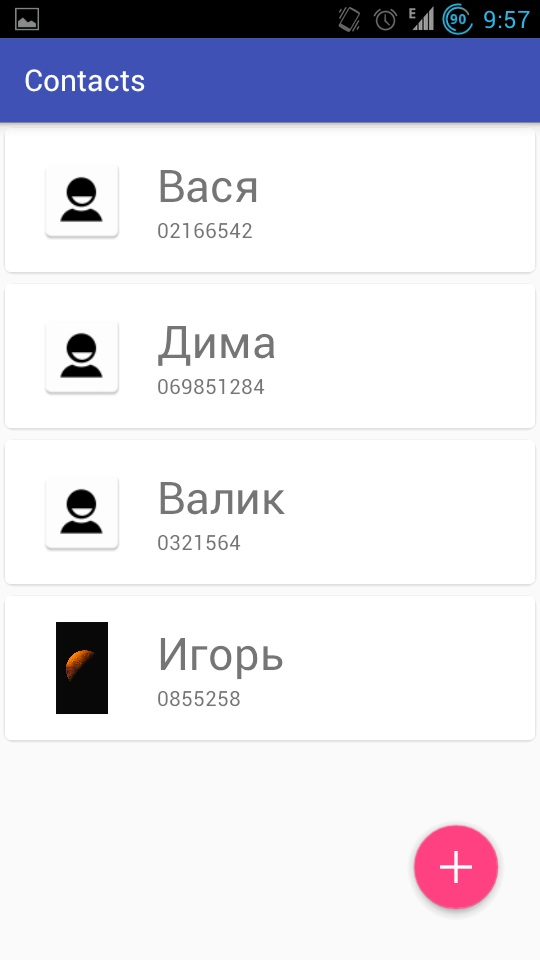
\includegraphics[width=1\linewidth]{images/3.jpg}}
	\caption{Результат добавления пользователя}
	\label{ris:image}
\end{figure}
\hfill
\begin{figure}[h]
	\center{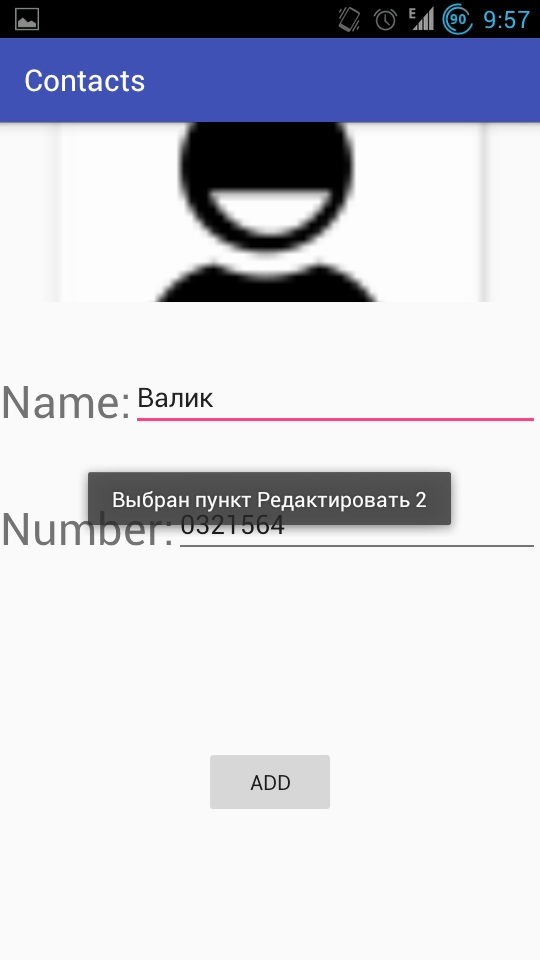
\includegraphics[width=1\linewidth]{images/4.jpg}}
	\caption{Редактирования данных пользователя}
	\label{ris:image}
\end{figure}

\clearpage